% ###########################################################
% ###########################################################
\ifFIGS
\begin{figure*}[!ht]
  \tikzexternalenable
    \tikzsetnextfilename{comorbidB}
  \vspace{-5pt}

\def\DATA{../../data_latest}
\iftikzX


\pgfplotsset{
    discard if/.style 2 args={
        x filter/.code={
            \edef\tempa{\thisrow{#1}}
            \edef\tempb{#2}
            \ifx\tempa\tempb
                \def\pgfmathresult{inf}
            \fi
        }
    },
    discard if not/.style 2 args={
        x filter/.code={
            \edef\tempa{\thisrow{#1}}
            \edef\tempb{#2}
            \ifx\tempa\tempb
            \else
                \def\pgfmathresult{inf}
            \fi
        }
    }
  }

  \begin{tikzpicture}[font=\bf\sffamily\fontsize{8}{10}\selectfont]
  \def\TEXTCOL{gray}
  \tikzset{
    hatch distance/.store in=\hatchdistance,
    hatch distance=20pt,
    hatch thickness/.store in=\hatchthickness,
    hatch thickness=2pt
  }


\pgfplotsset{
    accommodate labels/.code 2 args={
        \newlength{\myl}
        \pgfplotstableread{#1}\data
        \def\largestlength{0}
        \pgfplotstableforeachcolumnelement{#2}\of\data\as\cell{
            \settowidth{\myl}{\pgfinterruptpicture\cell\endpgfinterruptpicture}
            \pgfmathsetmacro\largestlength{max(\the\myl,\largestlength)}
        }
        \pgfplotsset{
            enlarge x limits={
                upper,              value=1/(1-(\largestlength+4pt)/\pgfkeysvalueof{/pgfplots/width})-1
            }
        }
    }
}

\def\COLDR{white}
\definecolor{alizarin}{rgb}{0.82, 0.1, 0.26}
\definecolor{amber}{rgb}{1.0, 0.75, 0.0}
\definecolor{amethyst}{rgb}{0.6, 0.4, 0.8}
\definecolor{apricot}{rgb}{0.98, 0.81, 0.69}
\definecolor{atomictangerine}{rgb}{1.0, 0.6, 0.4}
\definecolor{awesome}{rgb}{1.0, 0.13, 0.32}
\definecolor{azurec}{rgb}{0.0, 0.5, 1.0}
\definecolor{ballblue}{rgb}{0.13, 0.67, 0.8}
\definecolor{bittersweet}{rgb}{1.0, 0.44, 0.37}
\definecolor{bluem}{rgb}{0.0, 0.5, 0.69}
\definecolor{brightturquoise}{rgb}{0.03, 0.91, 0.87}

\def\COLBA{Red2}
\def\COLBB{Red3}
\def\COLBI{Red4}
\def\COLBG{DarkOrange2}
\def\COLBC{lightgray}
\def\COLBD{ballblue}
\def\COLBE{MidnightBlue}
\def\COLBF{SeaGreen3}
\def\COLBH{DarkSlateGray}
\def\COLBJ{bittersweet}
\def\COLBK{Orchid3}
\def\COLBL{black}
  
  % \makeatletter
  % \pgfdeclarepatternformonly[\hatchdistance,\hatchthickness]{flexible hatch}
  % {\pgfqpoint{0pt}{0pt}}
  % {\pgfqpoint{\hatchdistance}{\hatchdistance}}
  % {\pgfpoint{\hatchdistance-1pt}{\hatchdistance-1pt}}%
  % {
  %   \pgfsetcolor{\tikz@pattern@color}
  %   \pgfsetlinewidth{\hatchthickness}
  %   \pgfpathmoveto{\pgfqpoint{0pt}{0pt}}
  %   \pgfpathlineto{\pgfqpoint{\hatchdistance}{\hatchdistance}}
  %   \pgfusepath{stroke}
  % }
  % \makeatother
  % \pgfdeclarepatternformonly{north east lines wide}%
  % {\pgfqpoint{-1pt}{-1pt}}%
  % {\pgfqpoint{10pt}{10pt}}%
  % {\pgfqpoint{9pt}{9pt}}%
  % {
  %   \pgfsetlinewidth{0.4pt}
  %   \pgfpathmoveto{\pgfqpoint{0pt}{0pt}}
  %   \pgfpathlineto{\pgfqpoint{9.1pt}{9.1pt}}
  %   \pgfusepath{stroke}
  % }


  \def\COMPA{\DATA/figfiles/age_3_logodds_patternImmun.csv}
  \def\COMPB{\DATA/figfiles/age_3_logodds_patternnfect.csv}
  \def\COMPC{\DATA/figfiles/age_3_logodds_patternRespira.csv}
  \def\COMPD{\DATA/figfiles/age_3_logodds_patternCirculatory.csv} 
  \def\COMPINT{\DATA/figfiles/age_3_logodds_INTpattern.csv} 
 \def\MTYP{MImmun}
  \def\FTYP{FImmun}

  
  \def\WDTX{2.250in}
  \def\HGTX{3.75in}
  \def\HGTXB{5.65in}
  \def\HGTXC{6.25in}
  \def\HGTXD{2.5in}
  \def\HGTXE{4.325in}
  \def\OPC{1}
  \def\BWIDTH{6pt}
  \def\BWIDTHB{6pt}
  \clip (.75in,0.165in) rectangle (7.5in,-9.75in);


  
    \node [anchor=north west,align=left] (A) at (0,0.0) {
        \begin{tikzpicture}[text=\TEXTCOL]
%
%   \def\basis{1}
%   \pgfplotsset
%   {
%     x coord trafo/.code={\pgfmathparse{symlog(#1,\basis)}\pgfmathresult},
%     x coord inv trafo/.code={\pgfmathparse{symexp(#1,\basis)}\pgfmathresult},
%     xticklabel style={/pgf/number format/.cd,int detect,precision=2},
% } 


          \begin{axis}[legend style={anchor=east,at={(0.5,1.05)},inner sep=3pt,draw=none,fill=white,fill opacity=.850,align=right,text opacity=1,font=\bf\sffamily\fontsize{8}{9}\selectfont},axis line style={lightgray, opacity=0, thin},%
        enlargelimits=false,
        anchor=north west,
        height=\HGTX,
        width=\WDTX,
        %ymax=35,
        % xbar,
        ytick=data,% crucial line for the xticklabels directive 
        xmin=-2,
        %accommodate labels={\DISX}{description},
        yticklabels from table={\COMPA}{code},
        yticklabel style
        ={font=\bf\sffamily\fontsize{7}{7}\selectfont,
          align=right,rotate=0, text width=1.1in,
          anchor=east, yshift=0in,xshift=-.0450in,text=\TEXTCOL},
        major tick length=0pt,,text opacity=1,
        %xticklabel style=
        %{font=\bf\sffamily\fontsize{7}{7}\selectfont,
        %  text=\TEXTCOL},
        %grid,
        grid style={lightgray, dashed,opacity=.7},
        axis on top=false, bar width=\BWIDTH,
        xlabel={log odds ratio of normalized prevalence},
        scaled x ticks=false,
        xlabel style={yshift=0.05in,text=\TEXTCOL,text opacity=1},
        ylabel style={xshift=-.25in,yshift=0.075in,text=\TEXTCOL,text opacity=1},
        enlarge y limits=.04,
         x tick label style={/pgf/number format/fixed,/pgf/number format/precision=2,/pgf/number format/fixed zerofill,
     /pgf/number format/1000 sep = %\thinspace % Optional if you want to replace comma as the 1000 separator 
   },
   nodes near coords,visualization depends on={value \thisrow{negval}\as\rawx},
    every node near coord/.append style={anchor=west,align=left, text width=2in,font=\sffamily\rm\fontsize{8}{8}\selectfont,text=darkgray,text opacity=1,
        shift={(axis direction cs:-\rawx,0)}},
   point meta=explicit symbolic,ylabel={},
   , %xtick ={-0.03,0,0.03},
  % xmax=0.03,xmin=-0.03,
        ] 

        \addplot[draw=none,fill=none,xbar,area legend,opacity=0,text opacity=\OPC] table [ 
        y expr=\coordindex,
        x=pn,meta=description
        ] {\COMPA};

        \addplot[draw=\MXCOL,fill=\MXCOL,xbar,area legend,opacity=\OPC,text opacity=1] table [ 
        y expr=\coordindex,
        x=pn, discard if not={typ}{\MTYP}
        ] {\COMPA};
        \addplot[draw=\FXCOL,fill=\FXCOL,xbar,area legend,opacity=\OPC,text opacity=1] table [ 
        y expr=\coordindex,
        x=pn, discard if not={typ}{\FTYP}
        ] {\COMPA};

        
        % \addlegendentry{Female}
      \end{axis}
    \end{tikzpicture}};

      \node [anchor=north west,align=left] (B) at ([xshift=-1.68in,yshift=-0.0in]A.north east) {
        \begin{tikzpicture}[text=\TEXTCOL]
%
%   \def\basis{1}
%   \pgfplotsset
%   {
%     x coord trafo/.code={\pgfmathparse{symlog(#1,\basis)}\pgfmathresult},
%     x coord inv trafo/.code={\pgfmathparse{symexp(#1,\basis)}\pgfmathresult},
%     xticklabel style={/pgf/number format/.cd,int detect,precision=2},
% }


          \begin{axis}[legend style={anchor=east,at={(0.5,1.05)},inner sep=3pt,draw=none,fill=white,fill opacity=.85,align=right,text opacity=1,font=\bf\sffamily\fontsize{8}{9}\selectfont},axis line style={lightgray, opacity=0, thin},%
        enlargelimits=false,
        anchor=north west,
        height=\HGTXB,
        width=\WDTX,
        % xbar,
        ytick=data,% crucial line for the xticklabels directive 
        %xmin=0,
        %accommodate labels={\DISX}{description},
        yticklabels from table={\COMPB}{code},
        yticklabel style
        ={font=\bf\sffamily\fontsize{7}{7}\selectfont,
          align=right,rotate=0, text width=1.1in,
          anchor=east, yshift=0in,xshift=-.0450in,text=\TEXTCOL},
        major tick length=0pt,,text opacity=1,
        %xticklabel style=
        %{font=\bf\sffamily\fontsize{7}{7}\selectfont,
        %  text=\TEXTCOL},
        %grid
        grid style={lightgray, dashed,opacity=.7},
        axis on top=false, bar width=\BWIDTHB,
        xlabel={log odds ratio of normalized prevalence},
        scaled x ticks=false,
        xlabel style={yshift=0.05in,text=\TEXTCOL,text opacity=1},
        ylabel style={xshift=-2.25in,yshift=0.1in,text=\TEXTCOL,text opacity=1},
        enlarge y limits=.03,
         x tick label style={/pgf/number format/fixed,/pgf/number format/precision=2,/pgf/number format/fixed zerofill,
     /pgf/number format/1000 sep = %\thinspace % Optional if you want to replace comma as the 1000 separator 
   },
   nodes near coords,
       ,visualization depends on={value \thisrow{negval}\as\rawx},
    every node near coord/.append style={anchor=west,align=left, text width=2in,font=\sffamily\rm\fontsize{8}{8}\selectfont,text=darkgray,text opacity=1,
        shift={(axis direction cs:-\rawx,0)}},
   point meta=explicit symbolic,ylabel={ICD9 codes},
   , %xtick ={-0.03,0,0.03},
  % xmax=0.03,xmin=-0.03,
        ] 

        \addplot[draw=none,fill=none,xbar,area legend,opacity=0,text opacity=\OPC] table [ 
        y expr=\coordindex,
        x=pn, meta=description
        ] {\COMPB};

         
        \addplot[draw=\MXCOL,fill=\MXCOL,xbar,area legend,opacity=\OPC,text opacity=1] table [ 
        y expr=\coordindex,
        x=pn, discard if not={typ}{Mnfect}
        ] {\COMPB};

        
        \addplot[draw=\FXCOL,fill=\FXCOL,xbar,area legend,opacity=\OPC,text opacity=1] table [ 
        y expr=\coordindex,
        x=pn, discard if not={typ}{Fnfect}
        ] {\COMPB};

        
       \addplot[draw=\MXCOL,fill=\MXCOL,xbar,area legend,,postaction={
         pattern=flexible hatch,
        hatch distance=5pt,
        hatch thickness=1pt,
        draw=none,
        pattern color=gray, %ultra thick,
     },opacity=\OPC,text opacity=1] table [ 
        y expr=\coordindex,
        x=pn, discard if not={typ}{Mnfectv}
        ] {\COMPB};

        
        \addplot[draw=\FXCOL,fill=\FXCOL,xbar,area legend,postaction={
         pattern=flexible hatch,
        hatch distance=5pt,
        hatch thickness=1pt,
        draw=none,
        pattern color=black,  %ultra thick,
     },opacity=\OPC,text opacity=1] table [ 
        y expr=\coordindex,
        x=pn, discard if not={typ}{Fnfectv}
        ] {\COMPB};


        
        % \addlegendentry{Female}
      \end{axis}
    \end{tikzpicture}};

      \node [anchor=north west,align=left] (C) at ([yshift=-.2in]A.south west) {
        \begin{tikzpicture}[text=\TEXTCOL]
%
  \def\basis{1}
 %  \pgfplotsset
%   {
%     x coord trafo/.code={\pgfmathparse{symlog(#1,\basis)}\pgfmathresult},
%     x coord inv trafo/.code={\pgfmathparse{symexp(#1,\basis)}\pgfmathresult},
%     xticklabel style={/pgf/number format/.cd,int detect,precision=2},
% }


          \begin{axis}[legend style={anchor=east,at={(0.5,1.05)},inner sep=3pt,draw=none,fill=white,fill opacity=.85,align=right,text opacity=1,font=\bf\sffamily\fontsize{8}{9}\selectfont},axis line style={lightgray, opacity=0, thin},%
        enlargelimits=false,
        anchor=north west,
        height=\HGTXC,
        width=\WDTX,
        % xbar,
        ytick=data,% crucial line for the xticklabels directive 
        %xmin=0,
        %accommodate labels={\DISX}{description},
        yticklabels from table={\COMPC}{code},
        yticklabel style
        ={font=\bf\sffamily\fontsize{7}{7}\selectfont,
          align=right,rotate=0, text width=1.1in,
          anchor=east, yshift=0in,xshift=-.0450in,text=\TEXTCOL,text opacity=1},
        major tick length=0pt,
        %xticklabel style=
        %{font=\bf\sffamily\fontsize{7}{7}\selectfont,
        %  text=\TEXTCOL},
        %grid,
        grid style={lightgray, dashed,opacity=.7},
        axis on top=false, bar width=\BWIDTHB,
        xlabel={log odds ratio of normalized prevalence},
        scaled x ticks=false,
        xlabel style={yshift=0.05in,text=\TEXTCOL,text opacity=1},
        ylabel style={xshift=-.25in,yshift=0.075in,text=\TEXTCOL,text opacity=1},
        enlarge y limits=.03,
         x tick label style={/pgf/number format/fixed,/pgf/number format/precision=2,/pgf/number format/fixed zerofill,
     /pgf/number format/1000 sep = %\thinspace % Optional if you want to replace comma as the 1000 separator 
   },
    ,visualization depends on={value \thisrow{negval}\as\rawx},
    nodes near coords,
    every node near coord/.append style={%
       anchor=west, text width=2in,
      font=\sffamily\rm\fontsize{8}{8}\selectfont,text=darkgray,text opacity=1,
     shift={(axis direction cs:-\rawx,0)}
     },
     point meta=explicit symbolic,
    ylabel={},
   , %xtick ={-0.03,0,0.03},
  % xmax=0.03,xmin=-0.03,
        ] 

        \addplot[draw=none,fill=none,xbar,area legend,opacity=0,text opacity=\OPC] table [ 
        y expr=\coordindex,
        x=pn,meta=description
        ] {\COMPC};

        \addplot[draw=\MXCOL,fill=\MXCOL,xbar, area legend,opacity=\OPC,text opacity=1] table [ 
        y expr=\coordindex,
        x=pn, discard if not={typ}{MRespira}
        ] {\COMPC};
        \addplot[draw=\FXCOL,fill=\FXCOL,xbar,area legend,opacity=\OPC,text opacity=1] table [ 
        y expr=\coordindex,
        x=pn, discard if not={typ}{FRespira}
        ] {\COMPC};

      \end{axis}
    \end{tikzpicture}};


%       \node [anchor=north west,align=left] (D) at ([yshift=-.3in]B.south west) {
%         \begin{tikzpicture}[text=\TEXTCOL]
% %
%   \def\basis{1}
%  %  \pgfplotsset
% %   {
% %     x coord trafo/.code={\pgfmathparse{symlog(#1,\basis)}\pgfmathresult},
% %     x coord inv trafo/.code={\pgfmathparse{symexp(#1,\basis)}\pgfmathresult},
% %     xticklabel style={/pgf/number format/.cd,int detect,precision=2},
% % }


%           \begin{axis}[legend style={anchor=east,at={(0.5,1.05)},inner sep=3pt,draw=none,fill=white,fill opacity=.85,align=right,text opacity=1,font=\bf\sffamily\fontsize{8}{9}\selectfont},axis line style={lightgray, opacity=0, thin},%
%         enlargelimits=false,
%         anchor=north west,
%         height=\HGTXD,
%         width=\WDTX,
%         % xbar,
%         ytick=data,% crucial line for the xticklabels directive 
%         %ymax=15,
%         %accommodate labels={\DISX}{description},
%         yticklabels from table={\COMPD}{code},
%         yticklabel style
%         ={font=\bf\sffamily\fontsize{7}{7}\selectfont,
%           align=right,rotate=0, text width=1.1in,
%           anchor=east, yshift=0in,xshift=-.0450in,text=\TEXTCOL,text opacity=1},
%         major tick length=0pt,
%         %xticklabel style=
%         %{font=\bf\sffamily\fontsize{7}{7}\selectfont,
%         %  text=\TEXTCOL},
%         %grid,
%         grid style={lightgray, dashed,opacity=.7},
%         axis on top=false, bar width=\BWIDTHB,
%         xlabel={log odds ratio of normalized prevalence},
%         scaled x ticks=false,
%         xlabel style={yshift=0.05in,text=\TEXTCOL,text opacity=1},
%         ylabel style={xshift=-.25in,yshift=0.075in,text=\TEXTCOL,text opacity=1},
%         enlarge y limits=.04,
%          x tick label style={/pgf/number format/fixed,/pgf/number format/precision=2,/pgf/number format/fixed zerofill,
%      /pgf/number format/1000 sep = %\thinspace % Optional if you want to replace comma as the 1000 separator 
%    },
%     ,visualization depends on={value \thisrow{negval}\as\rawx},
%     nodes near coords,
%     every node near coord/.append style={%
%        anchor=west, text width=2in,
%       font=\sffamily\rm\fontsize{8}{8}\selectfont,text=darkgray,text opacity=1,
%      shift={(axis direction cs:-\rawx,0)}
%      },
%      point meta=explicit symbolic,
%     ylabel={},
%    , %xtick ={-0.03,0,0.03},
%   % xmax=0.03,xmin=-0.03,
%         ] 

%         \addplot[draw=none,fill=none,xbar,area legend,opacity=0,text opacity=\OPC] table [ 
%         y expr=\coordindex,
%         x=pn,meta=description
%         ] {\COMPD};

%         \addplot[draw=\MXCOL,fill=\MXCOL,xbar,postaction={
%          pattern=flexible hatch,
%         hatch distance=5pt,
%         hatch thickness=1pt,
%         draw=none,
%         pattern color=gray, %ultra thick,
%      }, area legend,opacity=\OPC,text opacity=1] table [ 
%         y expr=\coordindex,
%         x=pn, discard if not={typ}{MCirculatory}
%         ] {\COMPD};
%         \addplot[draw=\FXCOL,fill=\FXCOL,xbar,area legend,opacity=\OPC,text opacity=1] table [ 
%         y expr=\coordindex,
%         x=pn, discard if not={typ}{FCirculatory}
%         ] {\COMPD};

%       \end{axis}
%     \end{tikzpicture}};


      \node [anchor=north west,align=left] (D) at ([yshift=-.225in]B.south west) {
        \begin{tikzpicture}[text=\TEXTCOL]
%
  \def\basis{1}
 %  \pgfplotsset
%   {
%     x coord trafo/.code={\pgfmathparse{symlog(#1,\basis)}\pgfmathresult},
%     x coord inv trafo/.code={\pgfmathparse{symexp(#1,\basis)}\pgfmathresult},
%     xticklabel style={/pgf/number format/.cd,int detect,precision=2},
% }
\def\COMPX{\COMPINT}

          \begin{axis}[legend style={anchor=east,at={(0.5,1.05)},inner sep=3pt,draw=none,fill=white,fill opacity=.85,align=right,text opacity=1,font=\bf\sffamily\fontsize{8}{9}\selectfont},axis line style={lightgray, opacity=0, thin},%
        enlargelimits=false,
        anchor=north west,
        height=\HGTXE,
        width=\WDTX,
        % xbar,
        ytick=data,% crucial line for the xticklabels directive 
        %ymax=20,
        %accommodate labels={\DISX}{description},
        yticklabels from table={\COMPX}{code},
        yticklabel style
        ={font=\bf\sffamily\fontsize{7}{7}\selectfont,
          align=right,rotate=0, text width=1.1in,
          anchor=east, yshift=0in,xshift=-.0450in,text=\TEXTCOL,text opacity=1},
        major tick length=0pt,
        %xticklabel style=
        %{font=\bf\sffamily\fontsize{7}{7}\selectfont,
        %  text=\TEXTCOL},
        %grid,
        grid style={lightgray, dashed,opacity=.7},
        axis on top=false, bar width=\BWIDTHB,
        xlabel={log odds ratio of normalized prevalence},
        scaled x ticks=false,
        xlabel style={yshift=0.05in,text=\TEXTCOL,text opacity=1},
        ylabel style={xshift=-.25in,yshift=0.075in,text=\TEXTCOL,text opacity=1},
        enlarge y limits=.04,
         x tick label style={/pgf/number format/fixed,/pgf/number format/precision=2,/pgf/number format/fixed zerofill,
     /pgf/number format/1000 sep = %\thinspace % Optional if you want to replace comma as the 1000 separator 
   },
    ,visualization depends on={value \thisrow{negval}\as\rawx},
    nodes near coords,
    every node near coord/.append style={%
       anchor=west, text width=2in,
      font=\sffamily\rm\fontsize{8}{8}\selectfont,text=darkgray,text opacity=1,
     shift={(axis direction cs:-\rawx,0)}
     },
     point meta=explicit symbolic,
    ylabel={},
   , %xtick ={-0.03,0,0.03},
  % xmax=0.03,xmin=-0.03,
        ] 

        \addplot[draw=none,fill=none,xbar,area legend,opacity=0,text opacity=\OPC] table [ 
        y expr=\coordindex,
        x=pn,meta=description
        ] {\COMPX};

        \addplot[draw=\MXCOL,fill=\MXCOL,xbar, area legend,opacity=\OPC,text opacity=1] table [ 
        y expr=\coordindex,
        x=pn, discard if not={typ}{M}
        ] {\COMPX};
        \addplot[draw=\FXCOL,fill=\FXCOL,xbar,area legend,opacity=\OPC,text opacity=1] table [ 
        y expr=\coordindex,
        x=pn, discard if not={typ}{F}
        ] {\COMPX};

      \end{axis}
    \end{tikzpicture}};


    \node[] (T) at ([xshift=-1.4in,yshift=1.25in]B.east) {
      \arrayrulecolor{white}
      \setlength\arrayrulewidth{2pt}
      \mnp{1in}{\fontsize{9}{8}\selectfont\color{\TEXTCOL}
        {\large \color{black} Gender}
        \vskip 1em
        \begin{tabular}{L{.1in}L{.50in}}  %0
          \tikz[baseline=-0.5ex]{\node[text height=.075in,text width=.1in,fill=\MXCOL,,label={[]0:Male}] {};} 
          \tikz[baseline=-0.5ex]{\node[text height=.075in,text width=.1in,fill=\FXCOL,,label={[]0:Female}] {};}\\\hline          \tikz[baseline=-0.5ex]{\node[text height=.075in,text width=.1in,fill=none,,postaction={
         pattern=flexible hatch,
        hatch distance=5pt,
        hatch thickness=1pt,
        draw=none,
        pattern color=gray, %ultra thick,
     },label={[align=left]0:Viral/Fungal\\Inf.}] {};} 
          \end{tabular}
        }
      };
  
 \node[anchor=south west,align=left] (LA) at ([xshift=1in,yshift=-0.10in]A.north west) {{\LARGE A.} Endocrine Nutritional  Metabolic  And Immunity Dis.
 };
  \node[anchor=north west,align=left] (LB) at ([xshift=1in,yshift=-0in]$(LA.north west)!(B.west)!(LA.north east)$) 
{{\LARGE C.} Infectious And Parasitic Diseases
};
 \node[anchor=south west,align=left] (LD) at ([xshift=0in,yshift=-.1in]$(LB.north west)!(D.north)!(LB.south west)$) 
{{\LARGE D.} Similar Dis. with Opposed Association};
  \node[anchor=south west,align=left] (LC) at ([xshift=0in,yshift=-.05in]$(LA.north west)!(C.north)!(LA.south west)$)
  {{\LARGE B.} Respiratory Disorders };
\end{tikzpicture}


\else
  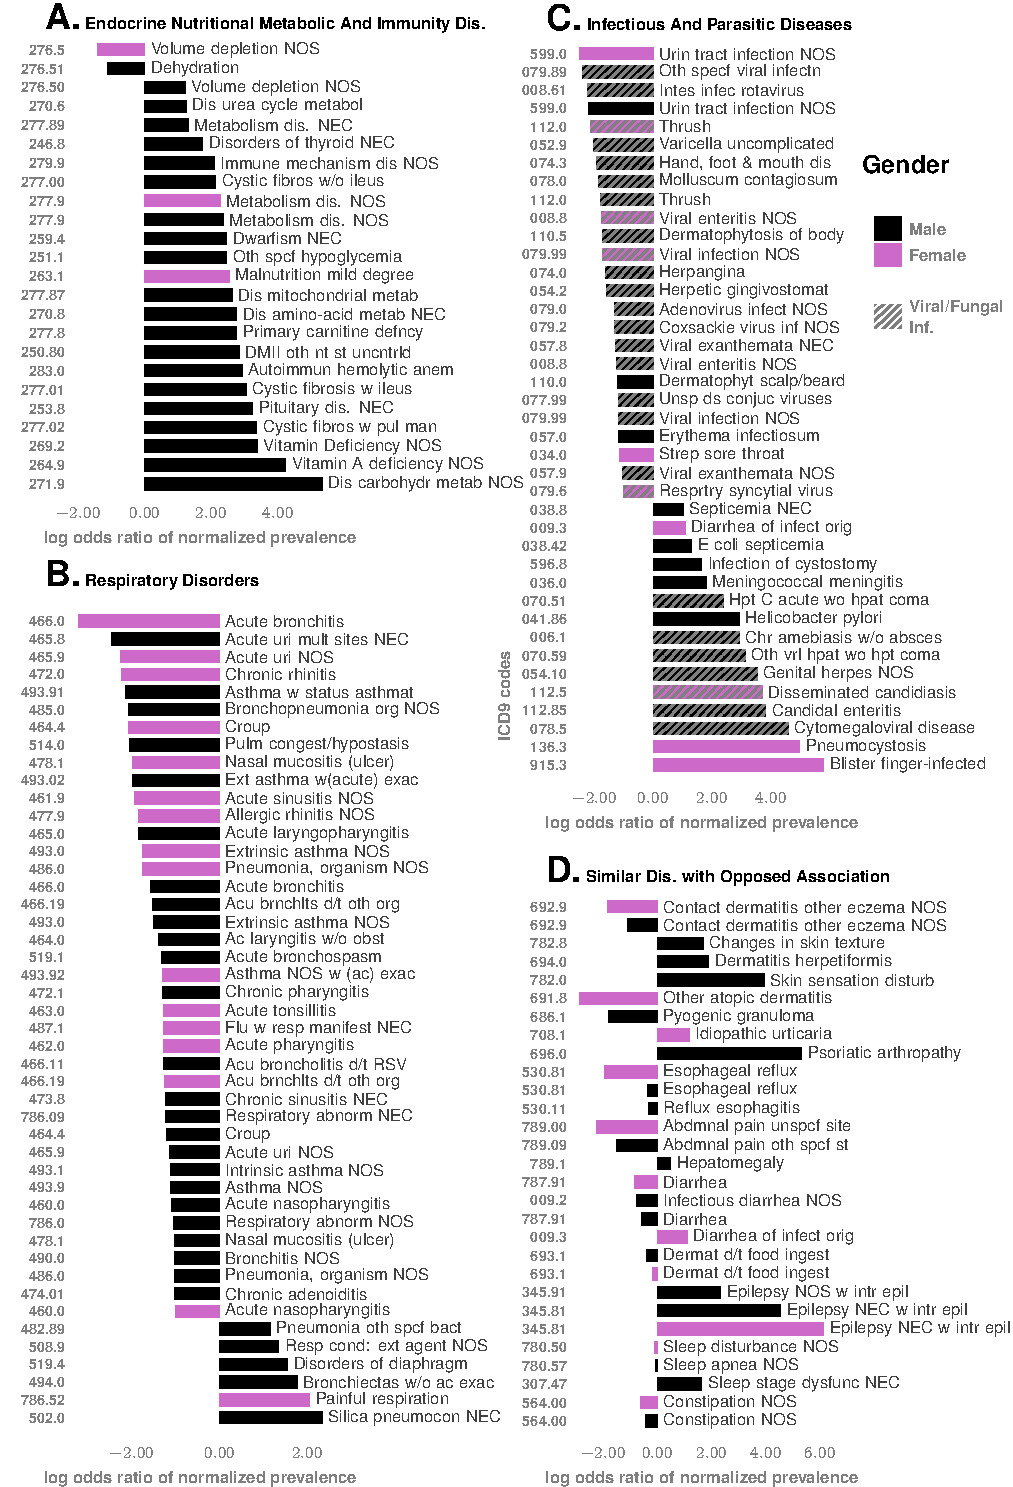
\includegraphics[width=0.8\textwidth]{Figures/External/comorbidB}
  \fi
  \vspace{-5pt}
  
  \captionN{\textbf{Details of Co-morbidity Patterns (at age $<3$ years)} for immunologic (panel A), respiratory (panel B), infections (panel C),  and disorders with similar pathobiology manifesting opposing association with autism (panel D).}\label{EXT-fig4}
    \vspace{-5pt}

\end{figure*}
\else
\refstepcounter{figure}\label{EXT-fig4}
\fi
%###########################################################
%###########################################################
% % ###########################################################
\ifFIGS
\begin{figure}[!ht]
  \tikzexternalenable
    \tikzsetnextfilename{comorbidC}

  \def\DATA{../../data_revision}

\iftikzX


\pgfplotsset{
    discard if/.style 2 args={
        x filter/.code={
            \edef\tempa{\thisrow{#1}}
            \edef\tempb{#2}
            \ifx\tempa\tempb
                \def\pgfmathresult{inf}
            \fi
        }
    },
    discard if not/.style 2 args={
        x filter/.code={
            \edef\tempa{\thisrow{#1}}
            \edef\tempb{#2}
            \ifx\tempa\tempb
            \else
                \def\pgfmathresult{inf}
            \fi
        }
    }
  }

  \begin{tikzpicture}[font=\bf\sffamily\fontsize{8}{10}\selectfont]
  \def\TEXTCOL{gray}
  \tikzset{
    hatch distance/.store in=\hatchdistance,
    hatch distance=20pt,
    hatch thickness/.store in=\hatchthickness,
    hatch thickness=2pt
  }


\pgfplotsset{
    accommodate labels/.code 2 args={
        \newlength{\myl}
        \pgfplotstableread{#1}\data
        \def\largestlength{0}
        \pgfplotstableforeachcolumnelement{#2}\of\data\as\cell{
            \settowidth{\myl}{\pgfinterruptpicture\cell\endpgfinterruptpicture}
            \pgfmathsetmacro\largestlength{max(\the\myl,\largestlength)}
        }
        \pgfplotsset{
            enlarge x limits={
                upper,              value=1/(1-(\largestlength+4pt)/\pgfkeysvalueof{/pgfplots/width})-1
            }
        }
    }
}

\def\COLDR{white}
\definecolor{alizarin}{rgb}{0.82, 0.1, 0.26}
\definecolor{amber}{rgb}{1.0, 0.75, 0.0}
\definecolor{amethyst}{rgb}{0.6, 0.4, 0.8}
\definecolor{apricot}{rgb}{0.98, 0.81, 0.69}
\definecolor{atomictangerine}{rgb}{1.0, 0.6, 0.4}
\definecolor{awesome}{rgb}{1.0, 0.13, 0.32}
\definecolor{azurec}{rgb}{0.0, 0.5, 1.0}
\definecolor{ballblue}{rgb}{0.13, 0.67, 0.8}
\definecolor{bittersweet}{rgb}{1.0, 0.44, 0.37}
\definecolor{bluem}{rgb}{0.0, 0.5, 0.69}
\definecolor{brightturquoise}{rgb}{0.03, 0.91, 0.87}

\def\COLBA{Red2}
\def\COLBB{Red3}
\def\COLBI{Red4}
\def\COLBG{DarkOrange2}
\def\COLBC{lightgray}
\def\COLBD{ballblue}
\def\COLBE{MidnightBlue}
\def\COLBF{SeaGreen3}
\def\COLBH{DarkSlateGray}
\def\COLBJ{bittersweet}
\def\COLBK{Orchid3}
\def\COLBL{black}
  
  \def\COMPA{\DATA/figfiles/Z2patternMental.csv}
  \def\COMPC{\DATA/figfiles/ZVplus.csv}
  \def\MTYP{MMental}
  \def\FTYP{FMental}
  \def\MTYPC{MV}
  \def\FTYPC{FV}


  
  \def\WDTX{2.20in}
  \def\HGTX{9.525in}
  \def\HGTXB{9.25in}
  \def\OPC{.9}
  \def\BWIDTH{10pt}
    \def\BWIDTHB{10pt}
  \def\BWIDTHC{7pt}  
  \clip (.85in,.3in) rectangle (7.5in,-9.25in);


  
    \node [anchor=north west,align=left] (A) at (0,0) {
        \begin{tikzpicture}[text=\TEXTCOL]
%
%   \def\basis{1}
%   \pgfplotsset
%   {
%     x coord trafo/.code={\pgfmathparse{symlog(#1,\basis)}\pgfmathresult},
%     x coord inv trafo/.code={\pgfmathparse{symexp(#1,\basis)}\pgfmathresult},
%     xticklabel style={/pgf/number format/.cd,int detect,precision=2},
% }


          \begin{axis}[yshift=1in,legend style={anchor=east,at={(0.5,2.75)},inner sep=3pt,draw=none,fill=white,fill opacity=.850,align=right,text opacity=1,font=\bf\sffamily\fontsize{8}{9}\selectfont},axis line style={lightgray, opacity=0, thin},%
        enlargelimits=false,
        anchor=north west,
        height=\HGTX,
        width=\WDTX,
        % xbar,
        ytick=data,% crucial line for the xticklabels directive 
        ymax=45, 
        %accommodate labels={\DISX}{description},
        yticklabels from table={\COMPA}{code},
        yticklabel style
        ={font=\bf\sffamily\fontsize{7}{7}\selectfont,
          align=right,rotate=0, text width=1.1in,
          anchor=east, yshift=0in,xshift=-.0450in,text=\TEXTCOL},
        major tick length=0pt,,text opacity=1,
        %xticklabel style=
        %{font=\bf\sffamily\fontsize{7}{7}\selectfont,
        %  text=\TEXTCOL},
        %grid,
        grid style={lightgray, dashed,opacity=.7},
        axis on top=false, bar width=\BWIDTH,
        xlabel={log odds ratio of normalized prevalence},
        scaled x ticks=false,
        xlabel style={yshift=0.3in,text=\TEXTCOL,text opacity=1},
        ylabel style={xshift=-.25in,yshift=0.075in,text=\TEXTCOL,text opacity=1},
        enlarge y limits=.05,
         x tick label style={/pgf/number format/fixed,/pgf/number format/precision=2,/pgf/number format/fixed zerofill,
           /pgf/number format/1000 sep = %\thinspace % Optional if you want to replace comma as the 1000 separator
          , yshift=0.21in,
   },
   nodes near coords,    ,visualization depends on={value \thisrow{negval}\as\rawx},
    every node near coord/.append style={anchor=west,align=left, text width=2in,font=\sffamily\rm\fontsize{8}{8}\selectfont,text=darkgray,text opacity=1,
        shift={(axis direction cs:-\rawx,0)}},
   point meta=explicit symbolic,ylabel={},
   , %xtick ={-0.03,0,0.03},
  % xmax=0.03,xmin=-0.03,
        ] 

        \addplot[draw=none,fill=none,xbar,area legend,opacity=0,text opacity=\OPC] table [ 
        y expr=\coordindex,
        x=pn,meta=description
        ] {\COMPA};

        \addplot[draw=\MXCOL,fill=\MXCOL,xbar,area legend,,postaction={
         pattern=flexible hatch,
        hatch distance=5pt,
        hatch thickness=1pt,
        draw=none,
        pattern color=gray, %ultra thick,
     },opacity=\OPC,text opacity=1] table [ 
        y expr=\coordindex,
        x=pn, discard if not={typ}{\MTYP}
        ] {\COMPA};
        \addplot[draw=\FXCOL,fill=\FXCOL,xbar,area legend,opacity=\OPC,text opacity=1] table [ 
        y expr=\coordindex,
        x=pn, discard if not={typ}{\FTYP}
        ] {\COMPA};

        
        % \addlegendentry{Female}
      \end{axis}
    \end{tikzpicture}};

      \node [anchor=north west,align=left] (B) at ([xshift=-1.55in,yshift=.01in]A.north east) {
        \begin{tikzpicture}[text=\TEXTCOL]
%
%   \def\basis{1}
%   \pgfplotsset
%   {
%     x coord trafo/.code={\pgfmathparse{symlog(#1,\basis)}\pgfmathresult},
%     x coord inv trafo/.code={\pgfmathparse{symexp(#1,\basis)}\pgfmathresult},
%     xticklabel style={/pgf/number format/.cd,int detect,precision=2},
% }


          \begin{axis}[legend style={anchor=east,at={(0.5,1.05)},inner sep=3pt,draw=none,fill=white,fill opacity=.85,align=right,text opacity=1,font=\bf\sffamily\fontsize{8}{9}\selectfont},axis line style={lightgray, opacity=0, thin},%
        enlargelimits=false,
        anchor=north west,
        height=\HGTXB,
        width=\WDTX,
        % xbar,
        % ymax=40,
        ymax=45,
        ytick=data,% crucial line for the xticklabels directive 
        %xmin=-2,
        %accommodate labels={\DISX}{description},
        yticklabels from table={\COMPC}{code},
        yticklabel style
        ={font=\bf\sffamily\fontsize{7}{7}\selectfont,
          align=right,rotate=0, text width=1.1in,
          anchor=east, yshift=0in,xshift=-.0450in,text=\TEXTCOL},
        major tick length=0pt,,text opacity=1,
        %xticklabel style=
        %{font=\bf\sffamily\fontsize{7}{7}\selectfont,
        %  text=\TEXTCOL},
        %grid
        grid style={lightgray, dashed,opacity=.7},
        axis on top=false, bar width=\BWIDTHB,
        xlabel={log odds ratio of normalized prevalence},
        scaled x ticks=false,
        xlabel style={yshift=0.03in,text=\TEXTCOL,text opacity=1},
        ylabel style={xshift=.25in,yshift=0.1in,text=\TEXTCOL,text opacity=1},
        enlarge y limits=.01,
         x tick label style={/pgf/number format/fixed,/pgf/number format/precision=2,/pgf/number format/fixed zerofill,
           /pgf/number format/1000 sep = %\thinspace % Optional if you want to replace comma as the 1000 separator
           , yshift=-0.05in
   },
   nodes near coords,    ,visualization depends on={value \thisrow{negval}\as\rawx},
    every node near coord/.append style={anchor=west,align=left, text width=2in,font=\sffamily\rm\fontsize{8}{8}\selectfont,text=darkgray,text opacity=1,
        shift={(axis direction cs:-\rawx,0)}},
   point meta=explicit symbolic,ylabel={ICD9 codes},
   , %xtick ={-0.03,0,0.03},
  % xmax=0.03,xmin=-0.03,
        ] 

        \addplot[draw=none,fill=none,xbar,area legend,opacity=0,text opacity=\OPC] table [ 
        y expr=\coordindex,
        x=pn, meta=description
        ] {\COMPC};

        \addplot[draw=\MXCOL,fill=\MXCOL,xbar,area legend,,postaction={
         pattern=flexible hatch,
        hatch distance=5pt,
        hatch thickness=1pt,
        draw=none,
        pattern color=gray, %ultra thick,
     },opacity=\OPC,text opacity=1] table [ 
        y expr=\coordindex,
        x=pn, discard if not={typ}{MV}
        ] {\COMPC};
        \addplot[draw=\FXCOL,fill=\FXCOL,xbar,area legend,opacity=\OPC,text opacity=1] table [ 
        y expr=\coordindex,
        x=pn, discard if not={typ}{FV}
        ] {\COMPC};

        
        % \addlegendentry{Female}
      \end{axis}
    \end{tikzpicture}};

%       \node [anchor=north west,align=left] (C) at ($(B.south west)!(A.north)!(B.north west)$) {
%         \begin{tikzpicture}[text=\TEXTCOL]
% %
% %   \def\basis{1}
% %   \pgfplotsset
% %   {
% %     x coord trafo/.code={\pgfmathparse{symlog(#1,\basis)}\pgfmathresult},
% %     x coord inv trafo/.code={\pgfmathparse{symexp(#1,\basis)}\pgfmathresult},
% %     xticklabel style={/pgf/number format/.cd,int detect,precision=2},
% % }


%           \begin{axis}[legend style={anchor=east,at={(0.5,1.05)},inner sep=3pt,draw=none,fill=white,fill opacity=.85,align=right,text opacity=1,font=\bf\sffamily\fontsize{8}{9}\selectfont},axis line style={lightgray, opacity=0, thin},%
%         enlargelimits=false,
%         anchor=north west,
%         height=\HGTXC,
%         width=\WDTX,
%         % xbar,
%         ytick=data,% crucial line for the xticklabels directive 
%         %xmin=0,
%         %accommodate labels={\DISX}{description},
%         yticklabels from table={\COMPC}{code},
%         yticklabel style
%         ={font=\bf\sffamily\fontsize{7}{7}\selectfont,
%           align=right,rotate=0, text width=1.1in,
%           anchor=east, yshift=0in,xshift=-.0450in,text=\TEXTCOL,text opacity=1},
%         major tick length=0pt,
%         %xticklabel style=
%         %{font=\bf\sffamily\fontsize{7}{7}\selectfont,
%         %  text=\TEXTCOL},
%         %grid,
%         grid style={lightgray, dashed,opacity=.7},
%         axis on top=false, bar width=\BWIDTHC,
%         xlabel={log odds ratio of normalized prevalence},
%         scaled x ticks=false,
%         xlabel style={yshift=0.05in,text=\TEXTCOL,text opacity=1},
%         ylabel style={xshift=-.25in,yshift=0.075in,text=\TEXTCOL,text opacity=1},
%         enlarge y limits=.03,
%          x tick label style={/pgf/number format/fixed,/pgf/number format/precision=2,/pgf/number format/fixed zerofill,
%      /pgf/number format/1000 sep = %\thinspace % Optional if you want to replace comma as the 1000 separator 
%    },
%    nodes near coords,    ,visualization depends on={value \thisrow{negval}\as\rawx},
%     every node near coord/.append style={anchor=west,align=left, text width=2in,font=\sffamily\rm\fontsize{8}{8}\selectfont,text=darkgray,text opacity=1,
%         shift={(axis direction cs:-\rawx,0)}},
%    point meta=explicit symbolic,ylabel={},
%    , %xtick ={-0.03,0,0.03},
%   % xmax=0.03,xmin=-0.03,
%         ] 

%         \addplot[draw=none,fill=none,xbar,area legend,opacity=0,text opacity=\OPC] table [ 
%         y expr=\coordindex,
%         x=pn,meta=description
%         ] {\COMPC};

%         \addplot[draw=\MXCOL,fill=\MXCOL,xbar,area legend,,postaction={
%          pattern=flexible hatch,
%         hatch distance=5pt,
%         hatch thickness=1pt,
%         draw=none,
%         pattern color=gray, %ultra thick,
%      },opacity=\OPC,text opacity=1] table [ 
%         y expr=\coordindex,
%         x=pn, discard if not={typ}{Merinatal}
%         ] {\COMPC};
%         \addplot[draw=\FXCOL,fill=\FXCOL,xbar,area legend,opacity=\OPC,text opacity=1] table [ 
%         y expr=\coordindex,
%         x=pn, discard if not={typ}{Ferinatal}
%         ] {\COMPC};

        
        % \addlegendentry{Female}
    %  \end{axis}
    %\end{tikzpicture}};
    \node[] (T) at ([xshift=-1.35in,yshift=2.5in]A.east) {
      \arrayrulecolor{white}
      \setlength\arrayrulewidth{2pt}
      \mnp{1in}{\fontsize{9}{8}\selectfont\color{\TEXTCOL}
        {\large \color{black} Gender}
        \vskip 1em
        \begin{tabular}{L{.1in}L{.5in}}
          \tikz[baseline=-0.5ex]{\node[text height=.075in,text width=.1in,fill=\MXCOL,,postaction={
         pattern=flexible hatch,
        hatch distance=5pt,
        hatch thickness=1pt,
        draw=none,
        pattern color=gray, %ultra thick,
     },label={[]0:Male}] {};} \\\hline  %0
          \tikz[baseline=-0.5ex]{\node[text height=.075in,text width=.1in,fill=\FXCOL,,label={[]0:Female}] {};} 
          \end{tabular}
        }
      };

  \node[anchor=south west,align=left] (LA) at ([xshift=1in,yshift=0in]A.north west) {{\LARGE A.} Mental Disorders };
  \node[anchor=south west,align=left] (LB) at ([xshift=3.5in,yshift=0in]$(LA.north west)!(A.north)!(LA.south west)$) {{\LARGE B.} Vaccinations \& Health Service Encounters};

 %  \node[anchor=south west,align=left] (LC) at ([xshift=3.5in,yshift=-4.5in]$(LA.north west)!(C.north)!(LA.south west)$) {{\LARGE C.} Digestive System Disorders
 % };
 
\end{tikzpicture}


\else
  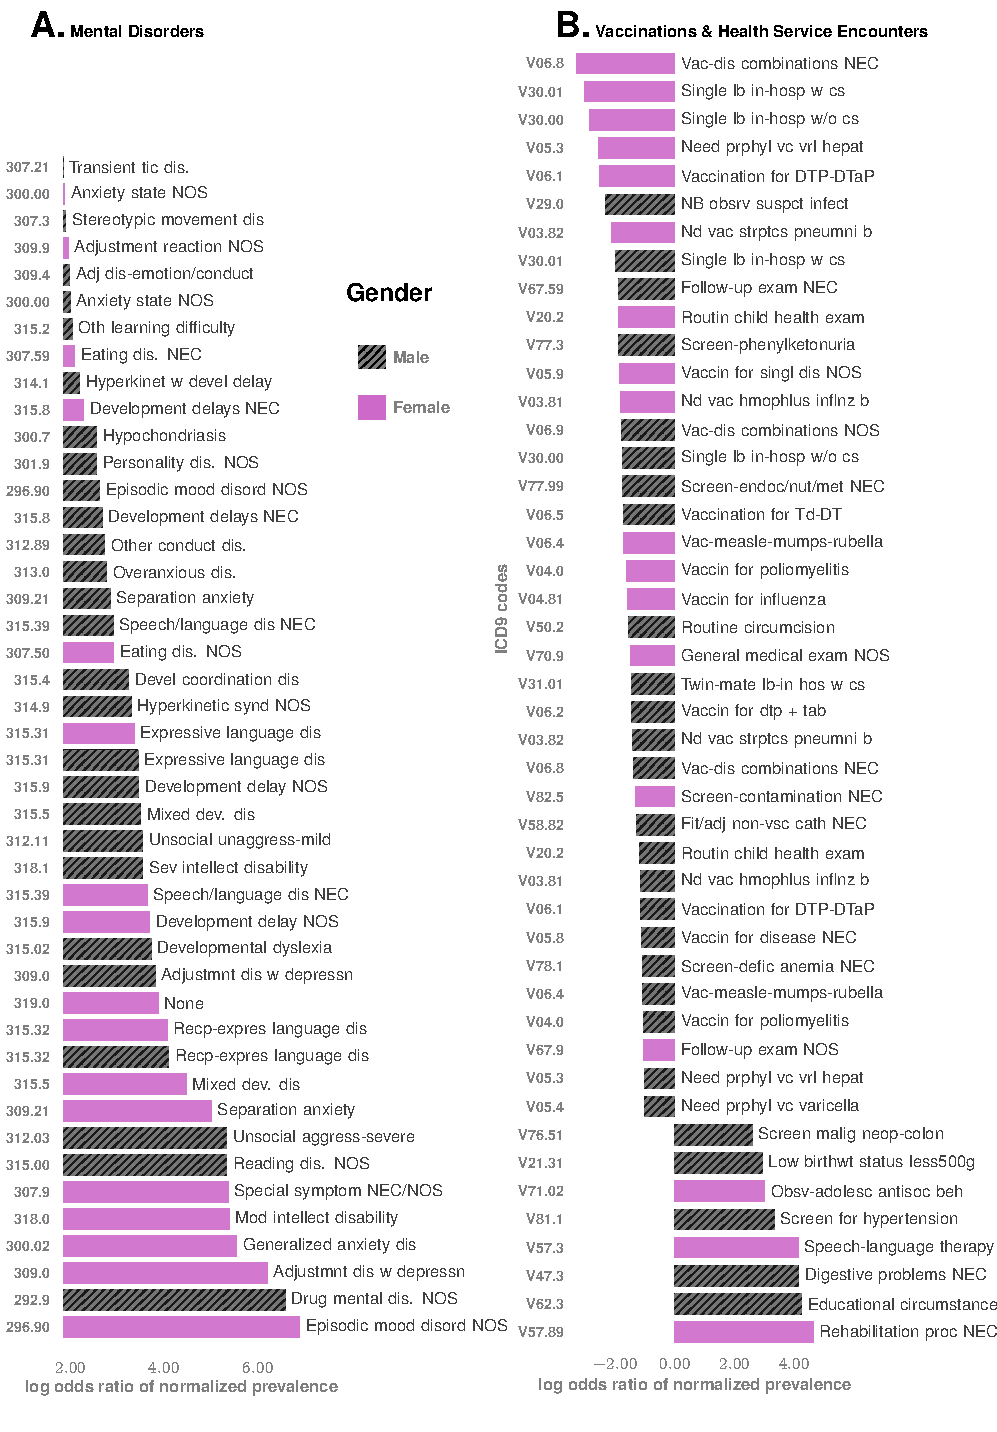
\includegraphics[width=0.9\textwidth]{Figures/External/comorbidC}
  \fi

  \vspace{-0pt}
  
  \captionN{\textbf{Co-morbidity Patterns}  for mental disorders, vaccinations and health-service encounters.}\label{EXT-figvv1}
\end{figure}%##########################################################
\else
\refstepcounter{figure}\label{EXT-figvv1}
\fi
% % % ###########################################################%
%###########################################################
%###############################################
%###########################################################
\ifFIGS
\begin{figure*}[!ht]
  \tikzexternalenable
    \tikzsetnextfilename{nopsych}
  \centering  
  \vspace{-10pt}
  
  \def\DATA{../../data_latest}
  \iftikzX
\begin{tikzpicture}[font=\bf\sffamily\fontsize{8}{10}\selectfont]
\def\TEXTCOL{gray}
    % \tikzset{
    %     hatch distance/.store in=\hatchdistance,
    %     hatch distance=20pt,
    %     hatch thickness/.store in=\hatchthickness,
    %     hatch thickness=2pt
    % }

% defining the new dimensions and parameters
\newlength{\hatchspread}
\newlength{\hatchthickness}
\newlength{\hatchshift}
\newcommand{\hatchcolor}{}
% declaring the keys in tikz
\makeatletter
\tikzset{hatchspread/.code={\setlength{\hatchspread}{#1}},
         hatchthickness/.code={\setlength{\hatchthickness}{#1}},
         hatchshift/.code={\setlength{\hatchshift}{#1}},% must be >= 0
         hatchcolor/.code={\renewcommand{\hatchcolor}{#1}}}
% setting the default values
\tikzset{hatchspread=3pt,
         hatchthickness=0.4pt,
         hatchshift=0pt,% must be >= 0
         hatchcolor=black}
% declaring the pattern
\pgfdeclarepatternformonly[\hatchspread,\hatchthickness,\hatchshift,\hatchcolor]% variables
   {custom north west lines}% name
   {\pgfqpoint{\dimexpr-2\hatchthickness}{\dimexpr-2\hatchthickness}}% lower left corner
   {\pgfqpoint{\dimexpr\hatchspread+2\hatchthickness}{\dimexpr\hatchspread+2\hatchthickness}}% upper right corner
   {\pgfqpoint{\dimexpr\hatchspread}{\dimexpr\hatchspread}}% tile size
   {% shape description
    \pgfsetlinewidth{\hatchthickness}
    \pgfpathmoveto{\pgfqpoint{0pt}{\dimexpr\hatchspread+\hatchshift}}
    \pgfpathlineto{\pgfqpoint{\dimexpr\hatchspread+0.15pt+\hatchshift}{-0.15pt}}
    \ifdim \hatchshift > 0pt
      \pgfpathmoveto{\pgfqpoint{0pt}{\hatchshift}}
      \pgfpathlineto{\pgfqpoint{\dimexpr0.15pt+\hatchshift}{-0.15pt}}
    \fi
    \pgfsetstrokecolor{\hatchcolor}
%    \pgfsetdash{{1pt}{1pt}}{0pt}% dashing cannot work correctly in all situation this way
    \pgfusepath{stroke}
   }
 \makeatother


%     \makeatletter
%     \pgfdeclarepatternformonly[\hatchdistance,\hatchthickness]{flexible hatch}
%     {\pgfqpoint{0pt}{0pt}}
%     {\pgfqpoint{\hatchdistance}{\hatchdistance}}
%     {\pgfpoint{\hatchdistance-1pt}{\hatchdistance-1pt}}%
%     {
%         \pgfsetcolor{\tikz@pattern@color}
%         \pgfsetlinewidth{\hatchthickness}
%         \pgfpathmoveto{\pgfqpoint{0pt}{0pt}}
%         \pgfpathlineto{\pgfqpoint{\hatchdistance}{\hatchdistance}}
%         \pgfusepath{stroke}
%     }
%     \makeatother
% \pgfdeclarepatternformonly{north east lines wide}%
%    {\pgfqpoint{-1pt}{-1pt}}%
%    {\pgfqpoint{10pt}{10pt}}%
%    {\pgfqpoint{9pt}{9pt}}%
%    {
%      \pgfsetlinewidth{0.4pt}
%      \pgfpathmoveto{\pgfqpoint{0pt}{0pt}}
%      \pgfpathlineto{\pgfqpoint{9.1pt}{9.1pt}}
%      \pgfusepath{stroke}
%     }


  \def\WDT{4.75in} 
  \def\WDTA{2in}    

  
  \def\datafile{\DATA/figfiles/AUC.csv}
  \def\datafileimp{\DATA/figfiles/AUC_imputed.csv}
 % \def\CHLM{Figures/augmented_M_fips_auc_rainbow}
 % \def\CHLF{Figures/augmented_F_fips_auc_rainbow}

  \def\CHLM{\DATA/figfiles/augmented_M_fips_auc_rainbow0}
  \def\CHLF{\DATA/figfiles/augmented_F_fips_auc_rainbow0}
  % \def\CHLM{Figures/augmented_M_fips_auc_Spectral_r0}
  % \def\CHLF{Figures/augmented_F_fips_auc_Spectral_r0}
  % \def\CHLM{Figures/augmented_M_fips_auc_Purples0}
  % \def\CHLF{Figures/augmented_F_fips_auc_Purples0}

  \def\ROCF{\DATA/figfiles/ROC_F_s.csv}
  \def\ROCM{\DATA/figfiles/ROC_M_s.csv}
  \def\IMP{\DATA/figfiles/importance20.csv}
 % \def\IMP{\DATA/figfiles/importance15.csv}
  \def\INTF{Figures/intf.dat}

  \def\HGT{1.30in}
  \def\WDT{6in}
  \def\WDTC{4in}
  \def\WDTR{1.9in}
  \def\WDTH{1.7in}
  
  \node[] (A) at (0,0) {};
  \node [anchor=north] (M) at (A.south) {\includegraphics[width=\WDTC]{\CHLM}};
  \node [anchor=north] (F) at ([yshift=-0.8in]M.south) {\includegraphics[width=\WDTC]{\CHLF}};
  
  % \begin{axis}[legend cell align=left,text=\TEXTCOL,
  %   legend style={text=black,anchor=east,at={(0.32,0.4)},inner sep=3pt,draw=none,fill=lightgray!10,fill opacity=.35,align=right,text opacity=1},
  %   name=E,
  %   at=(F.south west),
  %   xshift=0.6in,
  %   yshift=-0.7in,
  %   anchor=north west,
  %   width=\WDT,
  %   height=\HGT,
  %   ybar,
  %   bar width=4pt,
  %   xmin=.6,
  %   xmax=1,
  %   scale only axis=true, 
  %   axis on top=false,
  %   % axis background/.style={
  %   % shade,top color=transparent!15,bottom color=transparent!10},
  %   axis line style={lightgray!2, thin},
  %   grid,
  %   grid style={dashed,opacity=.95,thin,black!10},
  %   % xticklabel style={xshift=0.05in,yshift=-.05in},
  %   % xlabel style={xshift=-.075in,yshift=.05in,text=black},
  %   ylabel style={align=center,,text=black,anchor=center,
  %     yshift=-.1in,xshift=-.1in,font=\bf\sffamily\fontsize{7}{8}\selectfont,text=\TEXTCOL},
  %   % tickpos=left,
  %   ytick align=outside,
  %   xtick align=outside,
  %   major tick length=0pt,
  %   scaled y ticks = false,
  %   y tick label style={/pgf/number format/fixed,
  %     /pgf/number format/1000 sep = \thinspace % Optional if you want to replace comma as the 1000 separator 
  %   },
  %   ylabel={probability},
  %   ytick={0,0.02,0.04,0.06,0.08},
  %   ]
  %   \addplot [draw=none, thin, fill=\FXCOL,,fill opacity=1,, area legend]table [col sep=comma,x=AUC,y=F, area legend] {\datafileimp};
  %   \addlegendentry{AUC (Female)};
  %   \addplot [draw=none, thin, fill=\MXCOL,fill opacity=1, area legend] table [col sep=comma,x=AUC,y=M, area legend] {\datafileimp};
  %   \addlegendentry{AUC (Male)};
  %   % \draw[very thick,Red2] (axis cs:0.677,\pgfkeysvalueof{/pgfplots/ymin}) -- (axis cs:0.677,\pgfkeysvalueof{/pgfplots/ymax}) node [midway,right,fill=white,fill opacity=.9,text opacity=1,inner sep=2pt,pos=0.2,font=\sffamily\fontsize{6}{6}\selectfont] {0.677};
  %   % \draw[very thick,Red2] (axis cs:0.73,\pgfkeysvalueof{/pgfplots/ymin}) -- (axis cs:0.73,\pgfkeysvalueof{/pgfplots/ymax}) node [midway,right,fill=white,fill opacity=.9,text opacity=1,inner sep=2pt,pos=0.2,font=\sffamily\fontsize{6}{6}\selectfont] {0.73};
  % \end{axis}
  
  \node [anchor=north east, align=left,align=left] (B) at ([xshift=-0.35in,yshift=0.1in]M.north west) {
    \begin{tikzpicture}[anchor=center]
    \begin{axis}[legend cell align=left,text=\TEXTCOL, legend style={text=black,anchor=east,at={(1,0.12)},inner sep=1pt,draw=none,fill=gray!19,fill opacity=.85,align=right,text opacity=1,font=\bf\sffamily\fontsize{7}{8}\selectfont},
    name=K,
    clip=false,
    %at=(CC.center),
    xshift=-0in,
    yshift=-.25in,
    anchor=center,
    width=\WDTR,
    height=\WDTH,
    scale only axis=true,
    enlargelimits=false,
    axis on top=false,
     axis background/.style={
     shade,top color=transparent!0,bottom color=transparent!15},
    axis line style={black!2, very thick},
    grid,
    grid style={opacity=.9,thin,black!20},
    % xticklabel style={xshift=0.05in,yshift=-.05in},
    xlabel style={yshift=.05in,text=\TEXTCOL},
    ylabel style={align=center,,text=\TEXTCOL,anchor=center,
      yshift=-.175in},
    % tickpos=left,
    ytick align=outside,
    xtick align=outside,
    major tick length=0pt,
    scaled y ticks = false,
    y tick label style={/pgf/number format/fixed,
      /pgf/number format/1000 sep = \thinspace % Optional if you want to replace comma as the 1000 separator 
    },
    ylabel={TPR},xlabel={FPR},
    xmin=-0.05,
    ymax=1.02,
    extra x ticks={1},extra x tick labels={1}]
%
    \def\LCOL{Red1}
        \addplot [name path=a,smooth,draw=\FXCOL, ultra thick, fill=none,, pattern color=\FXCOL,pattern=custom north west lines,hatchspread=6pt,hatchthickness=3pt,fill opacity=.35,hatchcolor=Orchid3!60]table [col sep=comma,x=fpr ,y=tpr] {\ROCF};
          \addlegendentry{Female (AUC 81.6\%)}
  \addplot [smooth,draw=\MXCOL, ultra thick, fill=none,fill opacity=.5,]table [col sep=comma,x=fpr ,y=tpr] {\ROCM};
    \addlegendentry{Male (AUC 84.4\%)} 


\draw[name path=b,smooth,draw=\LCOL,,,very thick] (axis cs:0.05,0) -- (axis cs:0.05,\pgfkeysvalueof{/pgfplots/ymax})
      %\addplot [name path=b,smooth,draw=\LCOL,,,very thick]table [col sep=comma,x=fpr ,y=tpr] {\INTF} 
node [fill=white,midway,sloped,above,right,pos=.725,yshift=-.165in,text=\LCOL,align=center,font=\bf\sffamily\fontsize{7}{8}\selectfont] {specificity \\95.0\%};
      %\draw[Red1,name path=b,] (axis cs:0.05,0) -- (axis cs:0.05,1);
      \fill [name intersections={of=a and b},Red1] (intersection-1) circle (2pt)coordinate (c) ;


      \draw [\LCOL,very thick] (c) -- ($(axis cs:\pgfkeysvalueof{/pgfplots/xmin},0)!(c)!(axis cs:\pgfkeysvalueof{/pgfplots/xmin},1)$) ;
      \draw [\LCOL,very thick] (c) -- ($(axis cs:1,0)!(c)!(axis cs:1,1)$)node [font=\bf\sffamily\fontsize{7}{8}\selectfont,fill=lightgray!50,midway,below,pos=.7,yshift=-.1in,xshift=-.1in,text=\LCOL] {sensitivity: 51.8\%\\PPV (Male): 15.8\%\\PPV (Female): 18.8\%};
      % \draw [black,name path=d] (axis cs:0,0.38) -- (axis cs:1,.38)node [midway,below,pos=.65] {M-CHAT/F 38.8\%};
      % \fill [name intersections={of=d and b},black] (intersection-1) circle (2pt)coordinate (dd) ;
      %\draw[ultra thin,dashed,black] (c) -- (axis cs:1,.5175);
    \end{axis}
    \end{tikzpicture} 
  };
%
  \node [anchor=north east,align=left] (R) at ([xshift=-1.55in,yshift=1in]F.north west) {

\begin{axis}[legend cell align=left,legend style={anchor=east,at={(.9,0.1)},inner sep=3pt,draw=none,fill=white,fill opacity=.85,align=right,text opacity=1,font=\bf\sffamily\fontsize{8}{9}\selectfont},axis line style={lightgray, opacity=0, thin},%
enlargelimits=true,
%grid,
xshift=.1in,
anchor=north west,
  height=4in,
width=2.15in,
    xbar, 
    ytick=data,% crucial line for the xticklabels directive 
    ymin=0, 
    yticklabels from table={\IMP}{feature},
        yticklabel style={font=\bf\sffamily\fontsize{7}{7}\selectfont,align=right,rotate=0, text width=1.1in, anchor=east, yshift=0in,xshift=-.045in,text=\TEXTCOL},
major tick length=0pt,
xticklabel style={font=\bf\sffamily\fontsize{7}{7}\selectfont,text=\TEXTCOL},
grid,
grid style={lightgray, opacity=.7},
axis on top=false, bar width=4.2pt,xlabel={importance},xlabel style={yshift=0.05in,text=\TEXTCOL},
enlarge y limits=0.03,
] 

\addplot[opacity=1,fill=\MXCOL, area legend] table [ 
    y expr=\coordindex,
    x=M
] {\IMP};   
\addlegendentry{Male}
\addplot[opacity=1,fill=\FXCOL, area legend] table [ 
    y expr=\coordindex,
    x=F
] {\IMP};   
\addlegendentry{Female}

\end{axis} 

  };

  \node[anchor=south west,align=left] (LA) at ([xshift=.2in,yshift=0in]M.north west) {{\LARGE C.} AUC Spatial Variation (Males)   };
  \node[anchor=south west,align=left] (LB) at ([xshift=.2in,yshift=0in]F.north west) {{\LARGE D.} AUC Spatial Variation (Females)   };
  %\node[anchor=south west,align=left] (LC) at ([xshift=0in,yshift=.1in]$(LA.west)!(E.north west)!(LB.west)$) {{\LARGE C.} AUC Distribution over US Counties};
  \node[anchor=north west,align=left] (LD) at ([xshift=-0in,yshift=0in]$(B.west)!(LA.north)!(B.north west)$) {{\LARGE A.} ROC Curves at $150$ weeks  };

  \node[anchor=south west,align=left] (LR) at ([xshift=-0in,yshift=0.05in]$(LD.north west)!(R.north)!(LD.south west)$) {{\LARGE B.} Top 20  Phenotype-specific Features };

\end{tikzpicture}

\else
  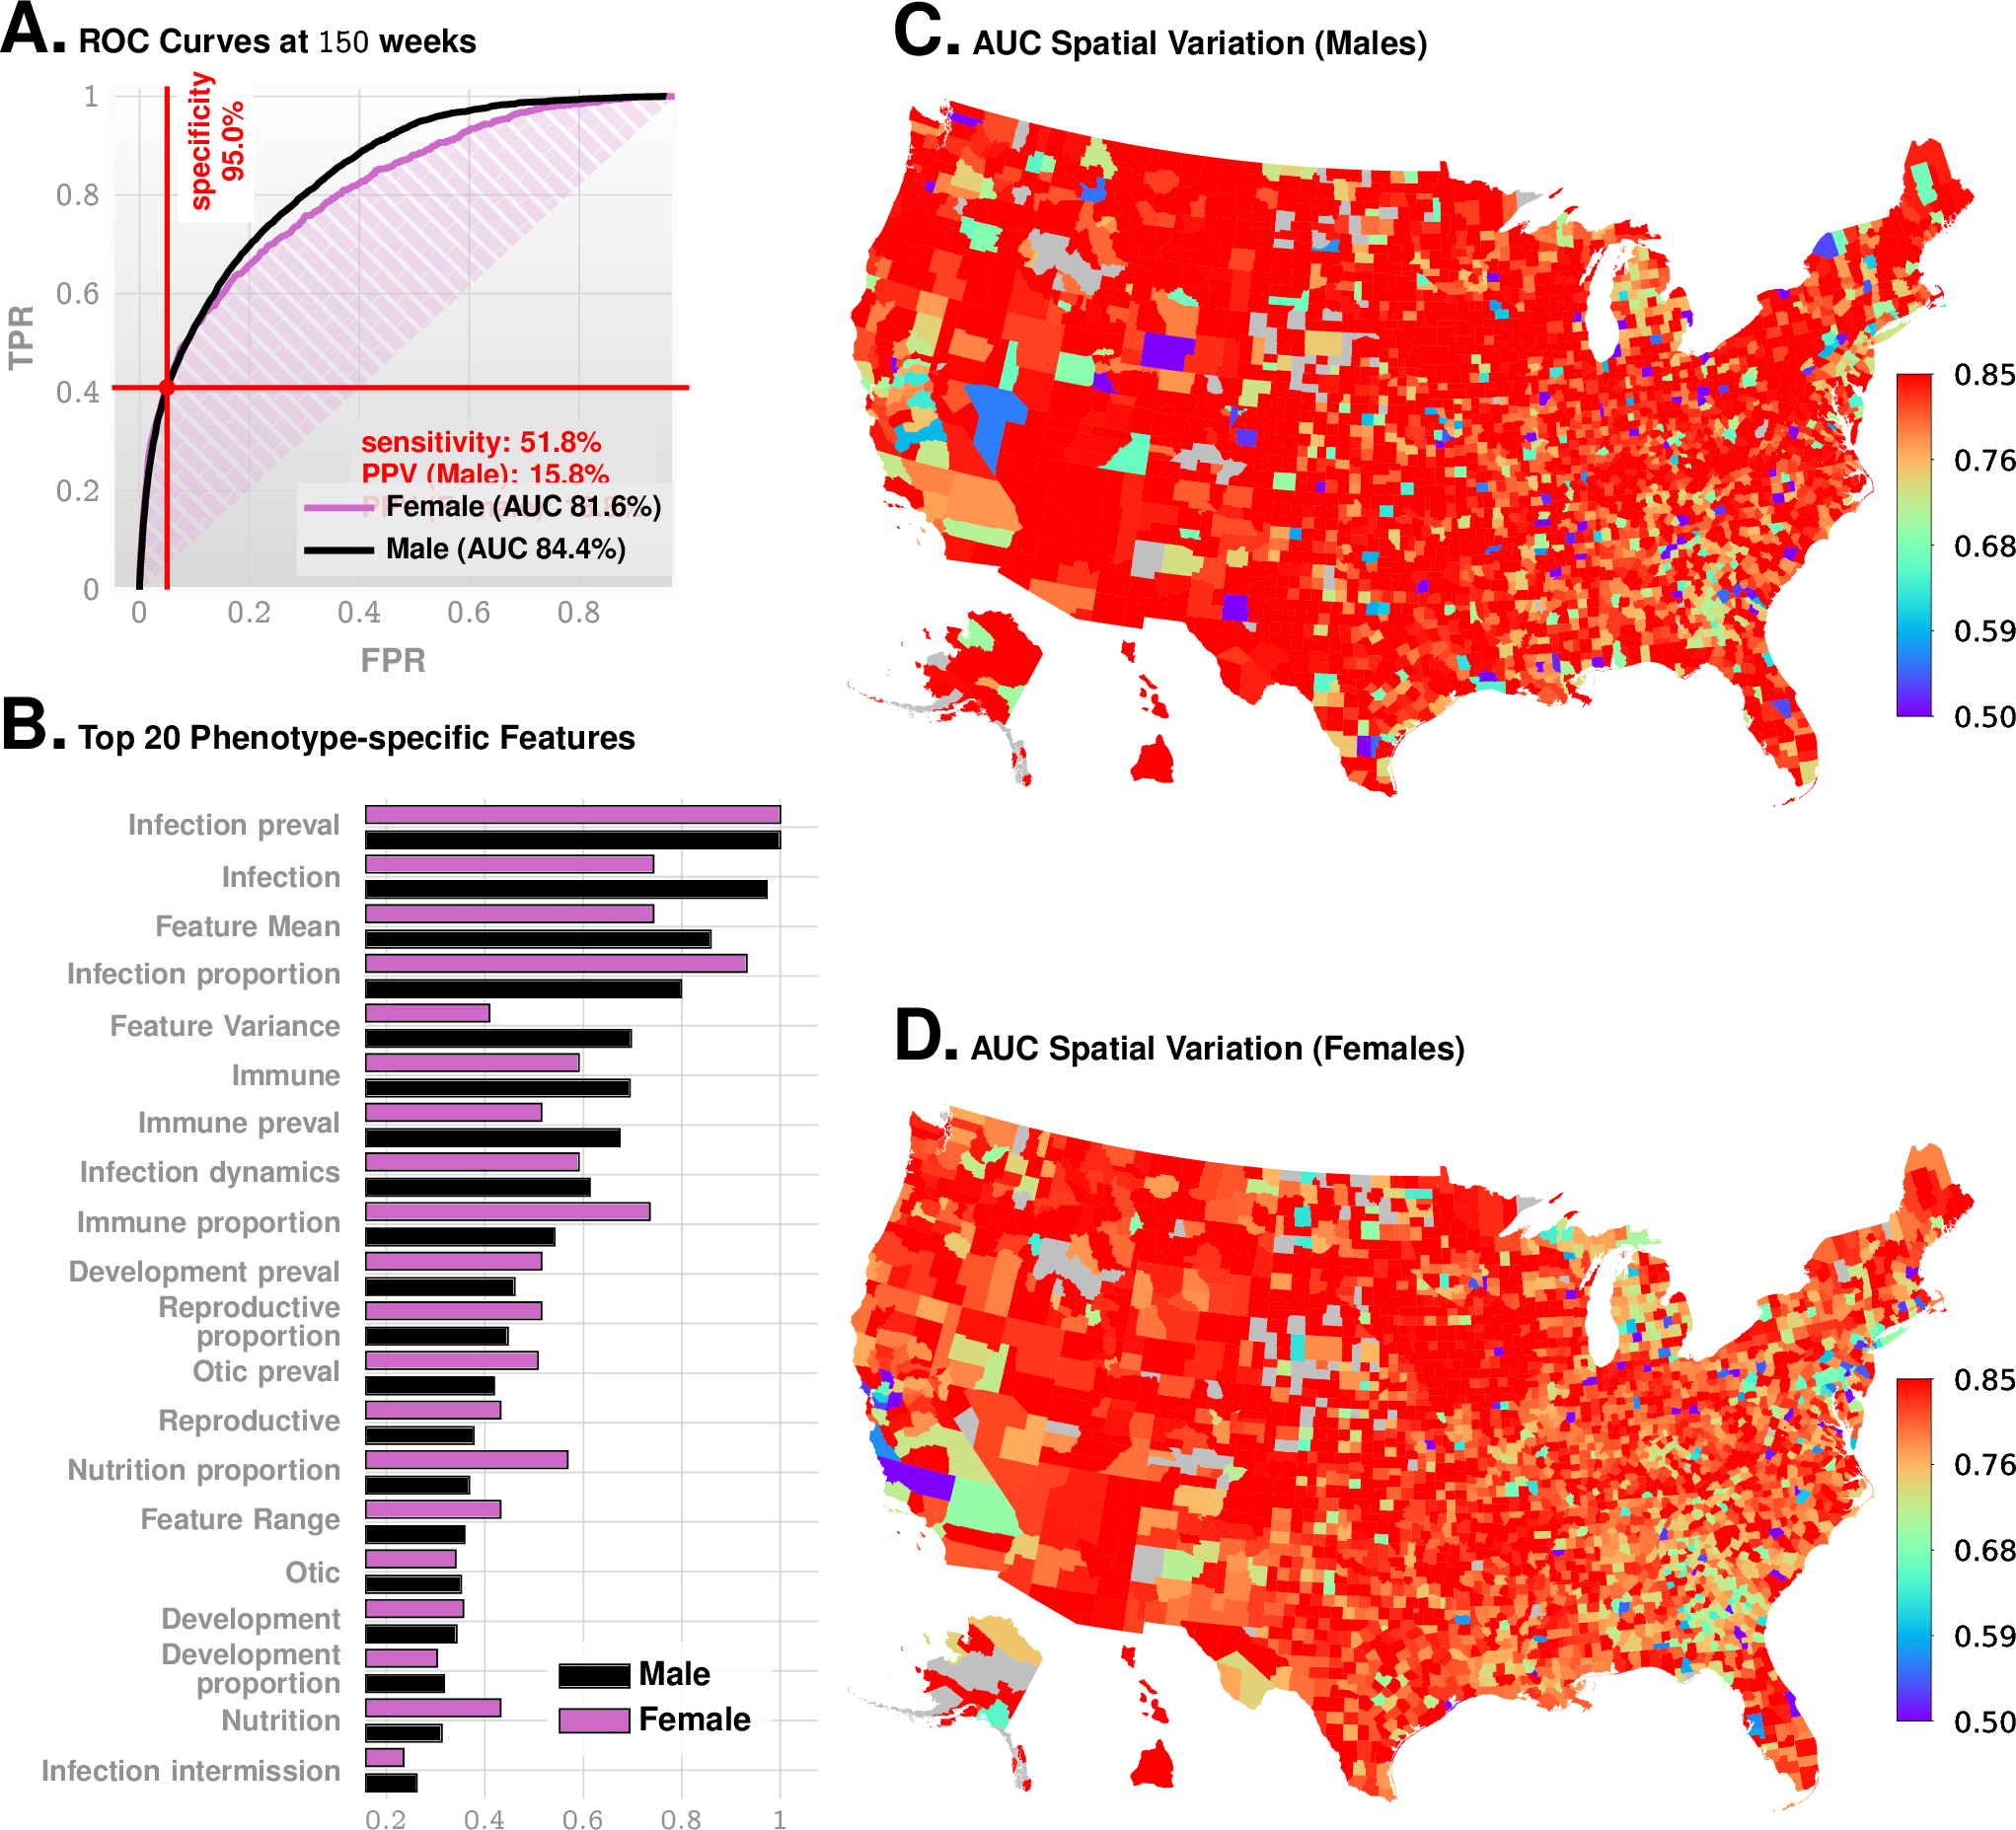
\includegraphics[width=0.95\textwidth]{Figures/External/nopsych}
  \fi 
     \vspace{-5pt}

     \captionN{Predictive Performance without psychiatric codes (ICD9 290 - 319)  and codes for health status and services (ICD9 V0-V91)  included. As shown, the performance is comparable at 150 weeks, with the AUC for females marginally lower (compare with Fig.~\ref{main-fig1} in the main text). The feature importances also are similar, with infectious diseases inferred to have the most importance (or weight) in the pipeline, which is also the case once we add psychiatric phenotypes, and codes for health services in our analysis. As shown in  SI-Fig.~\ref{EXT-figvv1}A, the psychiatric codes all increase risk, and the vaccination codes (See  SI-Fig.~\ref{EXT-figvv1}B) all decrease risk when those codes are included. This is why an alternate analysis was carried out to make sure that we are not picking up on psychiatric codes alone. Note in particular that the sensitivity/specificity point highlighted in panel A above is identical after adding the codes. This suggests that our predictive performance arises from patterns learned from co-morbidities, which are not just neuropsychiatric in nature.}\label{EXT-fig1nop}
\end{figure*}
\else
\refstepcounter{figure}\label{EXT-fig1nop}
\fi
% %###########################################################
